\documentclass{article}
\pdfpagewidth=8.5in
\pdfpageheight=11in

\usepackage{ijcai18}

\usepackage{times}
\usepackage{xcolor}
\usepackage{soul}
\usepackage[utf8]{inputenc}
\usepackage[small]{caption}

\usepackage{url}

\usepackage{booktabs} % For formal tables
\usepackage{amsmath}
\usepackage{amssymb}
\usepackage{amsthm}
\usepackage{indentfirst}
\usepackage{graphicx}
\usepackage{multirow}
\usepackage{makecell}
\usepackage{mathrsfs}
\usepackage{bbm}
\usepackage[linesnumbered,ruled]{algorithm2e}
\allowdisplaybreaks

\DeclareMathOperator*{\argmax}{arg\,max}

\newtheorem{theorem}{Theorem}[section]
\newtheorem{corollary}{Corollary}[theorem]
\newtheorem{definition}{Definition}[section]

\newcommand{\sumi}{\sum\limits_i}
\newcommand{\sumj}{\sum\limits_j}
\newcommand{\sumk}{\sum\limits_k}
\newcommand{\sumij}{\sum\limits_{ij}}

\newcommand{\sx}{x_{ij}}
\newcommand{\sbp}{bp_{ij}}

\newcommand{\sumijx}[1]{\sumij\sx{}#1}

\newcommand{\sProb}{Prob_i(\sbp)}
\newcommand{\sCost}{Cost_i(\sbp)}

\newcommand{\sV}{V_{ij}}
\newcommand{\sW}{W_{ij}^{(k)}}
\newcommand{\sB}{B^{(k)}}

\newcommand{\sBudget}{Budget^{(k)}}
\newcommand{\sROI}{ROI^{(k)}}

\newcommand{\inRange}[1]{\in\{1,2,...,#1\}}

\newcommand{\sCPP}{CPP_j}
\newcommand{\sCR}{CR_j}
\newcommand{\sPPI}{PPI_{ij}}
\newcommand{\sCPI}{RPI_{ij}}

\newcommand{\sRevenuePforP}{\sumijx{\sCPI\sProb}}
\newcommand{\sRevenuePforU}{\sumijx{(1+\sCR)\sCost}}
\newcommand{\sPerformance}{\sumijx{\sPPI\sProb}}
\newcommand{\sBiddingCost}{\sumijx{\sCost}}

\newcommand{\salpha}{\alpha^{(k)}}
\newcommand{\szeta}{\zeta^{(k)}}
\newcommand{\sbeta}{\beta_i}
\newcommand{\seta}{\eta_i}
\newcommand{\sgamma}{\gamma_{ij}}

\newcommand{\sF}{F_{ij}}
\newcommand{\sS}{S_{ij}}
\newcommand{\sG}{G_i}

\newcommand{\valpha}{\vec{\alpha}}
\newcommand{\vtheta}{\vec{\theta}}

\newcommand{\pprob}{\phi}
\newcommand{\pcost}{\psi}
\newcommand{\uff}{\mathscr{F}}
\newcommand{\uf}{f(bp; \pprob, \pcost, p(x))}

\newcommand{\dspresourceconstraint}{\sumij \sx \sW(\sbp) \le \sB}
\newcommand{\ammkpresourceconstraint}{\sumij \sx \sW(\sV) \le \sB}

\newcommand{\assignmentconstraint}{\sumj \sx \le 1}

\newcommand{\scoreconstraint}{\sbeta \ge \sS(\vec{\alpha})}

\newcommand{\linbp}{}
\newcommand{\ortbbp}{\sqrt{\frac{c\sCPI}{ROI}(1+\frac{1}{\lambda})+c^2}-c}
\newcommand{\dbbp}{\frac{\sCPI}{ROI}(1+\frac{1}{\alpha})}

\newcommand{\liniter}{\sbp^{'}=\frac{ActualROI_i(\sbp)}{ROI}Bid}
\newcommand{\ortbiter}{\lambda^{'}=\frac{ROI}{ActualROI(\lambda)}\lambda}
\newcommand{\dbiter}{\alpha^{'} = \frac{ROI}{ActualROI(\alpha)}\alpha}

\newcommand{\mr}[2]{\multirow{#1}{*}{#2}}
\newcommand{\mc}[2]{\multicolumn{#1}{c|}{#2}}

\title{Dual Based DSP Bidding Strategy and its Application}

%\author{
%Huahui Liu$^1$,
%Mingrui Zhu$^1$,
%Xiaonan Meng$^1$,
%Yi Hu$^1$,
%Hao Wang$^1$
%\\ 
%$^1$ Alibaba Group \\
%%
%\{
%huahui.lhh,
%mingrui.zmr,
%xiaonan.mengxn,
%erwin.huy,
%longran.wh
%\}@alibaba-inc.com
%}

\begin{document}

\maketitle

\begin{abstract}
In recent years, RTB(Real Time Bidding) becomes a popular online advertisement trading method.
During the auction, each DSP(Demand Side Platform) is supposed to
    evaluate the current opportunity and respond with an ad and the corresponding bid price.
It's essential for the DSP to find an optimal ad selection and bid price determination strategy
    which maximizes its revenue under the budget and the ROI(Return On Investment) constraints.
We solve this problem by
    formalizing the DSP problem as a constrained optimization problem,
    proving that this is a strong duality problem and deriving the corresponding dual base strategy.
Our strategy is verified through the simulation and outperforms the state-of-the-art strategies in the DSP of Alibaba.
To the best of our knowledge, our solution is the first dual based DSP bidding framework
    that is derived from the strict second price auction assumption and
    generally applicable to multiple ads with various constraints.
\end{abstract}

%\keywords{Computational Advertising, Real Time Bidding, Demand Side Platform, Bidding Strategy}

\section{Introduction} \label{Introduction}

In recent years, RTB(Real Time Bidding) becomes a popular online advertisement trading method.
There are three major roles in the market, namely the SSP(Supply Side Platform), the DSP(Demand Side Platform) and the AdX(Ad Exchange).
The SSP controls a huge amount of websites and earns money by supplying impression opportunities.
The DSP holds a lot of advertisers and makes profit through fulfilling their marketing demands.
And the AdX, an online advertisement exchange, docks SSPs and DSPs and holds auctions.

In a typical scenario, an audience visits one of the SSP's websites, then the AdX is informed and an auction is initiated.
The AdX broadcasts a bid request to DSPs and waits for a short time(e.g. 100ms).
Each DSP is supposed to evaluate the current opportunity and respond with an ad and the corresponding bid price.
The AdX gathers bid responses arriving before the deadline and determines the winner and its bidding cost.
Finally, the AdX notifies the SSP about the auction result and the SSP serves the winner's ad to the audience.

\begin{figure}[!h]
\centering
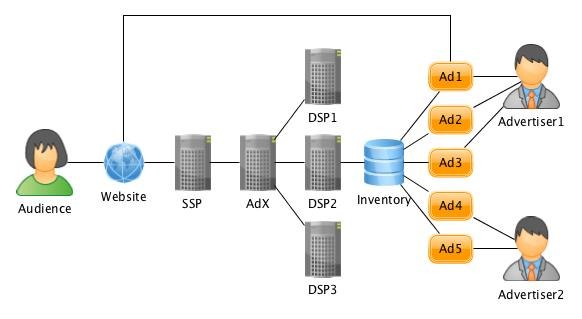
\includegraphics[width=1.0\linewidth]{./DSP.jpg}
\caption{Real Time Bidding}
\end{figure}

The advertiser should set the CPP(Cost Per Performance) and
    pay DSP the CPP times the units of performance delivered by the DSP(e.g. 1\$/click*10clicks=10\$).
DSP is interested in optimizing its own revenue earned from its advertisers.
During the optimization, both the budget and the ROI(Return On Investment) constraints must be satisfied.
The budget, set by the advertiser, is the maximum amount of money he is willing to spend in the DSP for a certain period of time (e.g. 100\$/day).
The ROI, lower bounded by DSP's operation team, is the revenue earned from its advertisers divided by the bidding cost payed to the AdX
    (e.g. ROI is 1.1 when DSP earns 110\$ and pays 100\$).

It's essential for the DSP to find an optimal ad selection and bid price determination strategy
    which maximizes its revenue under the budget and the ROI constraints.
We solve this problem by
    formalizing the DSP problem as a constrained optimization problem(Section \ref{Formalization}),
    proving that this is a strong duality problem and deriving the corresponding dual base strategy(Section \ref{Solution}).
Our strategy is verified through the simulation(Section \ref{Simulation}) and
    outperforms the state-of-the-art strategies in the DSP of Alibaba(Section \ref{Application}).

To the best of our knowledge, our solution is the first dual based DSP bidding framework
    that is derived from the strict second price auction assumption and
    generally applicable to multiple ads with various constraints.
These are the main contributions of this paper.

Before further discussion, it's worth to mention several points about our problem configuration.
First, the CPP is set on the ad level, i.e. the advertiser is able to set different CPPs for his ads.
Second, the constraints are set on the ad group level,
    e.g. the budget might be shared by the ads of the same advertiser
    and the DSP might be interested in controlling its global ROI.
Third, the PPI(Performance Per Impression) is defined as the expected performance of one impression with certain ad
    and its accurate prediction(\cite{Google2013}, \cite{Facebook2014}, \cite{FFM2016}, \cite{CVR}, \cite{DelayedFeedback})
    is of great importance in performance based advertising.
However, the PPI prediction is beyond the scope of this paper
    and we assume that the PPI is always explicitly provided in the rest of our discussion.
At last, given CPP and PPI, the RPI(Revenue Per Impression) is defined as the product of them
    and will be used extensively whenever the underlying factors are irrelevant.

\section{Related Works}

\cite{M6D} suggests a linear bidding strategy which, given the base bid price,
    bids in proportion to the relative quality of the impression.
However, their method is a heuristic one and lacks the theoretical foundations.

Based on the calculus of variations, \cite{WeinanZhang2014} suggests a non-linear relationship between the optimal bid price and the KPIs.
However, their strategy is derived from the first price auction assumption which doesn't hold in the RTB.
Besides, the winning rate is explicitly modeled as a function of the bid price.
To find the analytical solution of the optimal bid price,
    the winning rate function must be of specific forms,
    which makes their method inflexible.

Both the win rate and the winning price are estimated in \cite{XiangLi2014} and the corresponding bidding strategy is provided.
However, their strategy doesn't consider any constraints(e.g. budget) which are common in real applications.

While all the above researches consider only one campaign,
    \cite{WeinanZhang2015} extends \cite{WeinanZhang2014} and proposes a bidding strategy for multiple campaigns.
However, \cite{WeinanZhang2015} also shares the drawbacks of \cite{WeinanZhang2014} as listed above.

\cite{Joint2016} studies the joint optimization of multiple objectives with priorities.
\cite{Lift2016} argues that the bid price should be decided
    based on the performance lift rather than the absolute performance value.
The risk management of the RTB is discussed and a risk-aware bidding strategy is proposed in \cite{Risk2017}.
Through modeling the state transition of the auction competition,
    an optimal bidding policy is derived in \cite{Reinforce2017} based on the reinforcement learning theory.

%The probability estimation of interested feedbacks plays a central role in performance based advertising.
%CTR(Click Through Rate) prediction is of great importance and extensively studied by researchers.
%FTRL-Proximal, an online learning algorithm, is proposed in \cite{Google2013} and sparse model is learned for CTR prediction.
%In \cite{Facebook2014}, a hybrid model which combines decision trees with logistic regression
%    outperforms either of these methods on their own.
%In \cite{FFM2016}, field-aware factorization machines are used to predict CTR.
%Compared with clicks, the conversions are even more rare and harder to predict.
%To tackle the data sparseness, a hierarchical method is proposed in \cite{CVR} for CVR(Conversion Rate) prediction.
%Feedbacks are usually delayed in practice and \cite{DelayedFeedback} tries to
%    distinguish negative training samples without feedbacks eventually from those with delayed ones.

Bidding landscape is studied in \cite{YingCui2011} and log normal is used to model the distribution of the winning price.
\cite{Wu2015} predicts the win price with the censored data, which utilizes both the winning and the losing samples in the sealed auction.
%Traffic prediction is discussed in \cite{Traffic2016}.
Budget pacing is achieved through the throttling in \cite{Throttle2015} and the bid price adjustment in \cite{Pacing2013}.

Our work is mainly inspired by \cite{YeChen2011} in which the problem is modeled as a linear programming and
    the compact allocation strategy is derived from the complementary slackness.
Sealed second price auction is studied in \cite{SSPA1961}.
After all, the DSP problem is a sort of online matching problem and \cite{Mehta} is an informative survey of this area.

\section{Formalization} \label{Formalization}

\subsection{Primal} \label{Primal}

The DSP problem could be formalized into the standard problem as follows and the related symbols are explained in Table \ref{TableSymbols}.
Once we bid the $Impression$ with a $Ad$, it results in the gain $V$ and the resource consumptions $W$, both of which are functions of the $BidPrice$.
Our total gain should be maximized under the resource constraints $B$ with the $x$ and the $BidPrice$ as variables.
In addition, each $Impression$ should be distributed to no more than one $Ad$.
To conquer the computational hardness, the indicator variable $x$ is relaxed from $\{0, 1\}$ to $[0, 1]$.
Although most kinds of resources(e.g. budget) are private and only accessible to very limited number of $Ad$s in practice,
    we assume that, without loss of generality, all resources are public and shared by all $Ad$s.

\begin{alignat}{2}
    \max\limits_{\sx, \sbp} \quad & \sumij \sx \sV(\sbp) \quad    & {} \\
    \mbox{s.t.} \quad             & \dspresourceconstraint \quad  & \forall k \\
    \quad                         & \assignmentconstraint \quad   & \forall i \\
    \quad                         & \sx \ge 0 \quad               & \forall i,j
\end{alignat}

\begin{table}[h]
\caption{Symbols and Descriptions\label{TableSymbols}}
\begin{center}
\begin{tabular}{c|c}
\textbf{Symbol} & \textbf{Description} \\
\hline
\hline
$N$             & number of impressions \\
$M$             & number of ads \\
$K$             & number of resources \\
$i$             & index of the $Impression$ \\
$j$             & index of the $Ad$ \\
$k$             & index of the $Constraint$ \\
$\sbp$          & variable short for $BidPrice_{ij}$ \\
$\sV(bp)$       & gain function \\
$\sW(bp)$       & $k$-th resource consumption function \\
$\sB$           & $k$-th resource limit \\
\end{tabular}
\end{center}
\end{table}

The above formalization might seem too abstract to capture the details of
    those practical objective and constraints discussed in Section \ref{Introduction}.
To make things clearer, we
    derive the expected winning probability and the expected bidding cost
        under the second price auction assumption(Section \ref{SecondPriceAuction}),
    define the utility function family $\uff$ based on them(Section \ref{UtilityFunctionFamily})
    and show how to systematically encode those objective and constraints into the above formalization
        by setting $\sB$ and choosing $\sV(bp)$ and $\sW(bp)$ from $\uff$(Section \ref{ObjectivesAndConstraints}).

\subsection{Second Price Auction} \label{SecondPriceAuction}

Most AdXes adopt the sealed second price auction in which
    the DSP with the highest bid price wins and pays the amount of the second highest bid price.
For example, three DSPs bid 2\$, 1\$ and 3\$ respectively, so the third DSP wins and pays 2\$.
Furthermore, only the winner has access to the second highest bid price
    while the others observe nothing except the fact that they lose.

Due to the dynamic nature of the auction, the outcome is random.
To model this uncertainty, $p_i(x)$ is defined as the distribution of
    the highest bid price among all other DSPs' bid prices for the $Impression_i$ with support $[0, \infty)$.
In another word, the most competitive DSP will bid $x$ for the $Impression_i$ with probability $p_i(x) \mathrm{d} x$.

To win the $Impression_i$, our $BidPrice$ must be higher than $x$, but we will only pay $x$ eventually.
Then the expected winning probability and the expected bidding cost for our DSP could be defined as follows.
As our $BidPrice$ goes infinite, we'll win the $Impression_i$ with probability 1 and our bidding cost must be the mean of $p_i(x)$.

\begin{definition}
$Prob_i(BidPrice)= \int_0^{BidPrice} p_i(x) \mathrm{d} x$
\end{definition}

\begin{definition}
$Cost_i(BidPrice)= \int_0^{BidPrice} x p_i(x) \mathrm{d} x$
\end{definition}

It is the non-negativity of $p_i(x)$ and the integral forms of $Prob_i(BidPrice)$ and $Cost_i(BidPrice)$
    which play a central role in our theory(Section \ref{UtilityFunctionFamily}).
Except that, we make little, if any, assumption about the distribution family of $p_i(x)$.
In addition, in some special cases, even explicit modeling of $p_i(x)$ is unnecessary
    (Section \ref{DSPDualBasedStrategy} \& \ref{DSPNumericOptimization}), which simplifies the implementation of our strategy.
Whenever it is mandatory, $p_i(x)$ could be modeled with the method proposed by \cite{Wu2015}.

\subsection{Utility Function Family} \label{UtilityFunctionFamily}

The practical $V(bp)$ and $W(bp)$ in the DSP problem come from a certain family
    which is defined here and whose properties are shown without proof.

\begin{definition}
$\uff$ is the function family that $\forall f \in \uff$ is of the form
    $ \uf = \pprob Prob(bp) + \pcost Cost(bp) = \int_0^{bp} (\pprob + \pcost x)p(x)dx $.
\end{definition}

\begin{theorem} \label{ArgMaxTheorem}
Given $\forall f \in \uff$, we have $\argmax\limits_{bp} f = - \pprob / \pcost$.
\end{theorem}

\begin{theorem} \label{DerivationTheorem}
Given $\forall f \in \uff$, we have $f'=(\pprob + \pcost{}bp)p(bp)$.
\end{theorem}

\begin{theorem} \label{SecondDerivationTheorem}
Given $\forall g,h \in \uff$ with shared $p(x)$,
    we have $\frac{d^2h}{dg^2} = \frac{\pprob_g \pcost_h - \pcost_g \pprob_h}{(\pprob_g + \pcost_g bp)^3 p(bp)}$.
\end{theorem}

\begin{theorem} \label{ComparisonTheorem}
Given $\forall g,h \in \uff$ with shared $p(x)$ and $\pcost$, we have $\max\limits_{bp} g \ge \max\limits_{bp} f$
    if and only if $\pprob_g \ge \pprob_f$.
\end{theorem}

All the above theorems are listed here for summarization purpose and will be referenced when actually used.
It's safe to skip them now and come back later.

\subsection{Objective and Constraints} \label{ObjectivesAndConstraints}


The $\pprob$, $\pcost$ and $\sB$ for practical objective and constraints are listed in Table \ref{TableObjectives}.
It's straightforward to encode the revenue objective and the budget constraint into the standard form.
The ROI constraint, though not so obvious at the first glance, could be rewritten into the standard form as well.
By definition, we have
\begin{alignat}{1}
\frac{\sRevenuePforP}{\sBiddingCost}\ge\sROI
\end{alignat}
This formula could be transformed equivalently as
\begin{alignat}{1}
\sumijx{\{\sROI\sCost-\sCPI\sProb\}}\le0
\end{alignat}
Now it's easy to encode the ROI constraint into the standard form with $\pprob=-\sCPI$, $\pcost=\sROI$ and $\sB=0$.

\begin{table}
\caption{Practical Objective and Constraints\label{TableObjectives}}
\begin{center}
\begin{tabular}{c|c|c|c}
\textbf{Type}      & \boldmath{$\pprob$} & \boldmath{$\pcost$}  & \boldmath{$\sB$} \\
\hline
\hline
Revenue Objective  & $\sCPI$             & $0$                  & - \\
Budget Constraint  & $\sCPI$             & $0$                  & $\sBudget$ \\
ROI Constraint     & $-\sCPI$            & $\sROI$              & $0$ \\
\end{tabular}
\end{center}
\end{table}

\section{Solution} \label{Solution}

\subsection{Dual}

We define several basic functions and show the dual of the standard problem based on them.

\begin{definition}
$\sF(bp; \valpha) = \sV(bp) - \sumk \salpha \sW(bp)$
\end{definition}

\begin{definition}
$\sbp(\valpha) = \argmax\limits_{bp} \sF(bp; \valpha)$
\end{definition}

\begin{definition}
$\sS(\valpha) = \max\limits_{bp} \sF(bp; \valpha)$
\end{definition}

\begin{alignat}{2}
    \min\limits_{\salpha, \sbeta} \quad & \sumk \salpha \sB + \sumi \sbeta \quad & {} \\
    \mbox{s.t.} \quad                   & \scoreconstraint \quad                 & \forall i,j \\
    \quad                               & \salpha \ge 0 \quad                    & \forall k \\
    \quad                               & \sbeta \ge 0 \quad                     & \forall i
\end{alignat}

$\sF(bp; \valpha)$ serves as a scoring function which is used to estimate
    the utility of distributing the $Impression_i$ to the $Ad_j$ with bid price $bp$.
It could be interpreted as the compromised gain function in which
    our original gain $\sV(bp)$ is degenerated by the resource consumption $\sW(bp)$ times the opportunity price $\salpha$.
Since $\sF(bp; \valpha)$ is the linear combination of $\sV(bp)$ and $\sW(bp)$ from $\uff$ with shared $p_i(x)$,
    it must belong to $\uff$ too with its $\pprob_{\sF}$ and $\pcost_{\sF}$ as follows.
\begin{alignat}{2}
\pprob_{\sF}= & \pprob_{\sV} - \sum\limits_k \salpha \pprob_{\sW} \\
\pcost_{\sF}= & \pcost_{\sV} - \sum\limits_k \salpha \pcost_{\sW}
\end{alignat}
In practice, each ad is usually subjected to very limited number of constraints,
    which makes the calculation of $\pprob_{\sF}$ and $\pcost_{\sF}$ light-weighted.
What's more, according to Theorem \ref{ArgMaxTheorem}, $\sbp(\valpha)$ could be evaluated with the following equation.
\begin{alignat}{2}
\sbp(\valpha)= & - \pprob_{\sF} / \pcost_{\sF}
\end{alignat}

\subsection{Strong Duality}

It is provable that, as long as $\sW(bp)$ is convex function of $\sV(bp)$ for any $i$, $j$ and $k$,
    the strong duality of the standard problem(Section \ref{Primal}) holds.
The strict proof is omitted due to the limited space.
A less rigorous argument is that, since the standard problem could be seen as
    a relaxed MMKP(Multi-choice Multi-dimensional Knapsack Problem) with infinite many sub-choices $bp$,
    it must inherit the strong duality of the relaxed MMKP which is a linear programming.

\begin{theorem} \label{StrongDualityTheorem}
If $\sW(bp)$ is convex function of $\sV(bp)$ for any i, j and k, strong duality of the standard problem holds.
\end{theorem}

Due to the nice property of $\uff$, it's easy to check that,
    as to practical objective and constraints(Section \ref{ObjectivesAndConstraints}),
    $\sW(bp)$ is indeed convex function of $\sV(bp)$ for any $i$, $j$ and $k$,
    which immediately justifies the strong duality of the DSP problem.

\begin{theorem} \label{DSPStrongDualityTheorem}
Strong duality of the DSP problem holds.
\end{theorem}

\begin{proof}
According to Theorem \ref{DerivationTheorem}, we have $\sV'(bp)>0$ and $\sW(bp)$ must be function of $\sV(bp)$.
According to Theorem \ref{SecondDerivationTheorem}, we have $\frac{d^2\sW}{d\sV^2} \ge 0$ and $\sW(bp)$ must be convex function of $\sV(bp)$.
As a result, according to Theorem \ref{StrongDualityTheorem}, strong duality of the DSP problem holds.
\end{proof}

\subsection{Dual Based Strategy} \label{DSPDualBasedStrategy}

With strong duality satisfied, several important properties
    are claimed about the optimal solutions of both the primal and the dual problems
    (i.e. $\sx^*$, $\sbp^*$, $\valpha^*$ and $\sbeta^*$),
    based on which we propose the dual based strategy(Algorithm \ref{DSPAlgo}).

\begin{theorem}
$\sbp^* = \sbp(\valpha^*)$.
\end{theorem}

\begin{theorem}
$\sx^*(\sbeta^* - \sS(\valpha^*)) = 0$.
\end{theorem}

\begin{corollary}
If $\sS(\valpha^*) < 0$, $\sx^*$ must be $0$.
\end{corollary}

\begin{corollary}
If $S_{ij_1}(\valpha^*) < S_{ij_2}(\valpha^*)$, $x_{ij_1}^*$ must be $0$.
\end{corollary}

\begin{theorem}
$\sbeta^*(\sum\limits_j \sx^* - 1) = 0$.
\end{theorem}

\begin{corollary}
If $\exists j$ that $\sS(\valpha^*) > 0$, $\sum\limits_j \sx^*$ must be $1$.
\end{corollary}

\begin{algorithm}
\caption{Dual Based Strategy for DSP Problem \label{DSPAlgo}}

\For{$Impression_i \in \mathscr{I}$}
{
  \For{$Ad_j \in \mathscr{A}$}
  {
    $\pprob_{\sF} = \pprob_{\sV} - \sum\limits_k \salpha \pprob_{\sW}$

    $\pcost_{\sF} = \pcost_{\sV} - \sum\limits_k \salpha \pcost_{\sW}$

    $\sF(bp; \valpha^*) = \int_0^{bp} (\pprob_{\sF}+\pcost_{\sF}x)p_i(x)dx$

    $\sbp^* = \sbp(\valpha^*) = -\pprob_{\sF} / \pcost_{\sF}$

    $\sS^* = \sS(\valpha^*) = \max\limits_{bp} \sF(bp; \valpha^*)$
  }
  $j^* = \argmax\limits_j \sS^*$
  
  \If{$S_{ij^*}^* \ge 0$} { bid with ($Ad_{j^*}$, $bp_{ij^*}^*$) }
}
\end{algorithm}

In summary, given $Impression_i$, each $Ad_j$ should propose its own best score $\sS^*$ achieved by $\sbp^*$.
The $Impression_i$ should be awarded to the dominating $Ad_{j^*}$ if its best score $S_{ij^*}^*$ is positive
    and be discarded if that is negative.
Theoretically speaking, while most of which are determined by the above corollaries,
    behaviors remain undefined in two special cases.
First, there might be multiple dominating ads with the same best score.
Second, the best score of the dominating ad might be exactly zero.
In practice, however, both cases are probably rare due to the high resolution of impressions and ads and prone to cause relatively limited damage.
Ties could be broken randomly or by heuristics.

The $\sbp^*$ could be determined without $p_i(x)$ according to Theorem \ref{ArgMaxTheorem}.
In certain applications, $\pcost_{\sF}$ is the same for given $i$ and any $j$,
    then the $j^*$ could also be determined independent of $p_i(x)$ according to Theorem \ref{ComparisonTheorem}.
By disposing of $p_i(x)$ completely from the deciding process,
    it not only simplifies the computation, but also encourages the $p_i(x)$ free training process.

\subsection{Numeric Optimization} \label{DSPNumericOptimization}

During the execution of the dual base strategy,
    only the $\valpha^*$ is mandatory
    while the others(i.e. $\sx^*$, $\sbp^*$ and $\sbeta^*$) could be recovered from it,
    which makes our strategy storage efficient.
Next, we propose the numeric method to solve the $\valpha^*$.

\begin{definition}
$\sbeta(\valpha) = \max \{ 0, \sS(\valpha) \forall j \}$
\end{definition}

\begin{definition}
$\sG(\valpha) = \sum\limits_k \frac{\salpha \sB}{N} + \sbeta(\valpha)$
\end{definition}

By fixing $\valpha$ in the dual problem, the $\sbeta^*$ could be calculated as $\sbeta^* = \sbeta(\valpha)$.
Then the dual problem could be rewritten as
\begin{alignat}{2}
\min\limits_{\valpha \ge 0} & \sum\limits_i \sG(\valpha)
\end{alignat}
    and solved by SGD(Stochastic Gradient Descent).
Due to the convexity of the dual problem, it must converge to the global optimal $\valpha^*$.
This form also suggests that, the $\valpha^*$ depends on the distribution of the impressions as a whole
    rather than any specific sample.
Assuming the impressions within a small time window are i.i.d.,
    the $\valpha^*$ solved with the recent impressions could be reused in the near future.

It's provable that $\frac{\partial\sbeta(\valpha)}{\partial\salpha}$ must be
    either $-\sW(\sbp(\valpha))$ if the best score of the dominating $Ad_j$ is positive or $0$ otherwise.
This optimization method, though generally applicable, requires explicit modeling of $p_i(x)$.

The randomized version of $\sW(\sbp(\valpha))$ is observable during the execution of our strategy in the production environment.
Then the gradients could be approximated with these observations.
This optimization method is $p_i(x)$ free and much easier to implement.

\section{Simulation} \label{Simulation}

\subsection{Methodology}

To eliminate the uncertainty, our strategy is verified through simulation.
Two mocked ads $Ad_1$ and $Ad_2$ are created.
Three mocked constraints are listed in Table \ref{TableConstraints}.
Budgets of $Ad_1$ and $Ad_2$ are $20$ and $10$ respectively and the global ROI lower bound is $2$.
As suggested by \cite{YingCui2011}, $p(x)$ is assumed to be the log normal distribution $p(x;\mu,\sigma)$
    with the mean $\mu$ and the standard deviation $\sigma$ as parameters.
To mock the impressions, 200 tuples of $<\mu_i$, $\sigma_i$, $RPI_{i1}$, $RPI_{i2}>$ are drawn randomly.

\begin{table}
\caption{Mocked Constraints\label{TableConstraints}}
\begin{center}
\begin{tabular}{c|c|c|c}
\boldmath{$k$} & \textbf{Type}   & \textbf{Parameter}   & \textbf{Scope}   \\
\hline
\hline
$1$            & Budget          & $Budget^{(k)} = 20$ & $\{Ad_1\}$        \\
$2$            & Budget          & $Budget^{(k)} = 10$ & $\{Ad_2\}$        \\
$3$            & ROI             & $ROI^{(k)} = 2$     & $\{Ad_1, Ad_2\}$  \\
\end{tabular}
\end{center}
\end{table}

Once the configuration is ready, the $\valpha^*$ is solved by SGD(Section \ref{DSPNumericOptimization}).
After that, the dual based strategy is applied on the same configuration to recover the primal and the dual solutions.
Meanwhile, the consequent resource statistics are collected.

\subsection{Results and Analysis}

Both the primal and the dual objective values are approximately $2.164$ with negligible gap as claimed by Theorem \ref{DSPStrongDualityTheorem}.
All resources have non-negative surplus and no constraint is violated.
The resource statistics and the $\valpha^*$ are listed in Table \ref{TableStatisticsAndAlpha}.
As mentioned earlier, the $\alpha^*$ serves as so called the opportunity price of the resource.
Intuitively speaking, waste of resource with positive surplus shouldn't lead to any opportunity cost.
As a result, the corresponding $\alpha^*$ tends to be $0$.

\begin{table}[h]
\caption{Resource Statistics and $\alpha^*$\label{TableStatisticsAndAlpha}}
\begin{center}
\begin{tabular}{c|c|c|c|c}
\boldmath{$k$} & \textbf{Limit} & \textbf{Consumption} & \textbf{Surplus} & \boldmath{$\alpha^*$} \\
\hline
\hline
$1$            & $20.000$       & $0.865$              & $19.135$         & $0.000$ \\
$2$            & $10.000$       & $1.299$              & $8.701$          & $0.000$ \\
$3$            & $0.000$        & $0.000$              & $0.000$          & $4.749$ \\
\end{tabular}
\end{center}
\end{table}

\section{Application} \label{Application}

\subsection{Scenario}

We also deploy our strategy in the DSP platform of Alibaba.
In our application, the advertisers set budgets and pay for clicks, while the DSP is willing to maximize its revenue under the daily global ROI constraint.
There are so many ads in our inventory that it's impossible to go through each ad before the auction deadline.
Although these budgets are relatively small on average, they are quite large totally.

\begin{figure}[!h]
\centering
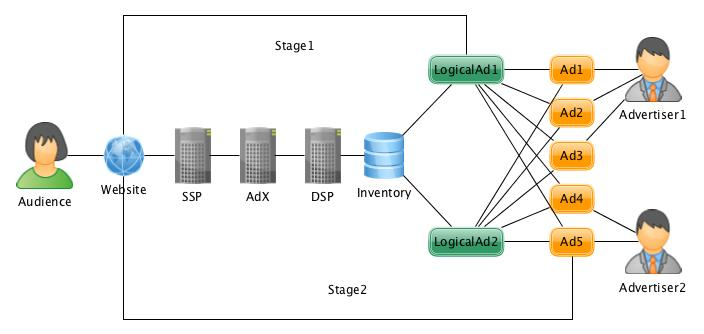
\includegraphics[width=1.0\linewidth]{./LogicalAd.jpg}
\caption{Real Time Bidding with Logical Ad}
\end{figure}

The RPI is predicted with well calibrated CPP and PPI predictors.
And to meet the latency requirement, the whole deciding process is decomposed into two stages with so called the logical ad.
The logical ad should be seen as the proxy of the physical ads and is binded with specific ad retrieval algorithm.
In the first stage, the DSP is supposed to make choices among just a few logical ads and respond in time.
In the second stage, once the chosen logical ad wins the auction, the physical ad is lazily retrieved with the corresponding algorithm.
Our logical ads are based on 4 heterogeneous ad retrieval algorithms whose details are omitted.
These algorithms are sorted by their historical performance in descending orders and 4 logical ads are constructed correspondingly.

In summary, our problem could be approximated as, given 4 logical ads with literally unlimited budget,
    maximizing the revenue under the daily global ROI constraint.
Since there is only one resource constraint, the superscript $k$ is omitted and
    the ROI is short for the global ROI in the rest of Section \ref{Application}.

According to our theory, we have $\pprob_{\sF}=(1+\alpha)\sCPI$ and $\pcost_{\sF}=-\alpha{}ROI$.
Since $\pcost_{\sF}$ is always $-\alpha{}ROI$, no $p_i(x)$ is required in the deciding process as discussed in Section \ref{DSPDualBasedStrategy}.
We could simply set $\sbp = \dbbp$ and bid in the AdX for the logical ad
    with the highest $\pprob_{\sF}$ or, equivalently, the highest $\sbp$.
To take full advantage of that, we adopt a simplified version of the $p_i(x)$ free optimization method
    suggested in Section \ref{DSPNumericOptimization}, i.e. $\dbiter$.

\subsection{Experiment Groups}

Our strategy is compared with a variation of the linear bidding strategy.
In \cite{M6D}, it's suggested that $\sbp=\frac{ActualCTR_{ij}}{CTR}Bid$ with the $Bid$ set by the operation team.
However, unlike the $ActualCTR_{ij}$ which is independent of $\sbp$, the $ActualROI_{ij}$ varies with it.
As a result, we iteratively update $\sbp$ with $\liniter$.

The optimal RTB theory is also applied to our application for comparison.
According to \cite{WeinanZhang2014}, we model the win probability as $w(bp;c)=\frac{bp}{c+bp}$ and bid with $\sbp=\ortbbp$,
    in which $c$ is fitted with the method proposed by \cite{Wu2015} and $\lambda$ is iteratively tuned with $\ortbiter$.

Four experiment groups are shown in Table \ref{TableExperimentGroups}.
The first three groups are designed to compare different strategies when applied to single logical ad,
    while the last group is used to test our strategy when applied to multiple logical ads.

\begin{table}
\caption{Experiment Groups\label{TableExperimentGroups}}
\begin{center}
\begin{tabular}{c|c|c}
\textbf{Group}    & \textbf{Inventory}         & \textbf{Period} \\
\hline
\hline
$LIN$    & $\{LogicalAd_1\}$                   & 24h \\
$ORTB$   & $\{LogicalAd_1\}$                   & 10min \\
$DB_{s}$ & $\{LogicalAd_1\}$                   & 10min \\
$DB_{m}$ & $\{LogicalAd_j|j \in \{1,2,3,4\}\}$ & 10min \\
\end{tabular}
\end{center}
\end{table}

All strategy parameters(i.e. $\sbp$, $\lambda$ and $\alpha$) are randomly initialized and
    iteratively adjusted with the actual ROI observed in the last period.
The period is set to 24 hours for the $LIN$ group due to the data sparseness
    and 10 minutes as to the others for robustness and faster convergence.
Note that the more frequent update introduces inexplicitly a 10 minutes ROI constraint
    which is stricter than the daily one and might degenerate the theoretical optimal.

To eliminate the potential bias, the experiment lasts for a whole ordinary week.
The bidding opportunities are distributed to each group randomly with equal probabilities.
For fairness, the same CPP and PPI predictors are shared by all groups.
The lower bound of the daily ROI is set to $3.5$.

\subsection{Results and Analysis}

The daily statistics of four metrics are plotted in Figure \ref{Result},
    namely the revenue, the actual ROI, the number of winning impressions and the revenue per winning impression.

\begin{figure}[!h]
\centering
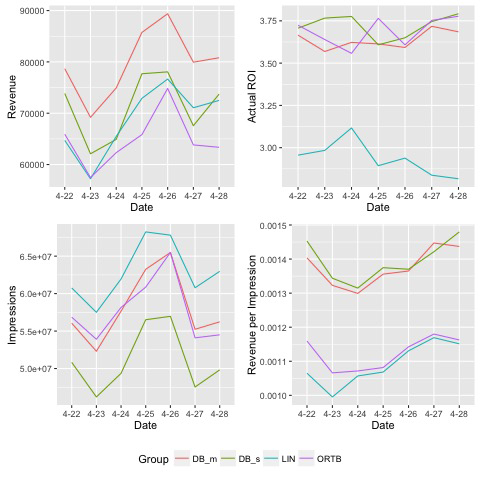
\includegraphics[width=1.0\linewidth]{./Result.jpg}
\caption{Experiment Results\label{Result}}
\end{figure}

Suffering from the stale data, the $LIN$ tends to
    earn less revenue than the others and violate the daily ROI constraint seriously,
    which makes it an inferior strategy.

While the daily ROI constraint is satisfied by both strategies,
    the $DB_s$ earns more revenue than the $ORTB$.
These two strategies are some how connected and share similar patterns in their bid price determination formulas.
Compared with the $DB_s$ who claims a linear relationship between the bid price and the expected revenue,
    the $ORTB$ suggests a non-linear one.
It prefers the impressions with lower expected revenue to those with higher expected revenue,
    which leads to more impressions and worse averaged quality.
The differences between the two strategies root from their different assumptions about the auction mechanism.
As a result, the $DB_s$ is superior practically and theoretically.

The $DB_m$, as an ensemble of four ad retrieval algorithms,
    achieves the most revenue without violation of the daily ROI constraint and becomes the best strategy.

\section{Conclusions and Future Works}

In this paper, we propose a dual based DSP bidding strategy
    derived from the second price auction assumption according to the convex optimization theory.
Our strategy is verified through the simulation and outperforms the state-of-the-art strategies in the DSP of Alibaba.
It's a theoretically solid and practically effective strategy with simple implementation and various applications.

Three problems remain unsolved and deserve further study.
First, is there a better way to solve the $\valpha^*$ of large scale in the dynamic environment?
On the one hand, in a typical DSP, there will be millions of constraints shared by similar number of ads.
Each of the constraints deserves a $\alpha$, which makes the vector $\valpha$ very large.
On the other hand, billions of impressions are broadcast by the AdX every day and bid by hundreds of DSPs simultaneously.
The bidding strategies are interactively adjusted by the DSPs and the inventories are frequently updated by the advertisers,
    which makes the bidding landscape unstable.
Both properties make the $\valpha^*$ hard to solve.

Second, how to construct and index the logical ads automatically in the massive ads applications, balancing the latency and the performance?
It's obvious that both the deciding and the training processes share the same ad evaluation and maximum determination style,
    which makes their computational complexities linearly related with the number of candidate logical ads.
At one extreme, each ad is represented by exactly one logical ad and the latency is unacceptable.
At the other extreme, all ads are represented by the only logical ad, while the performance might be seriously degenerated.
A proper compromise combined with the efficient indexing tricks will accelerate both processes by orders of magnitude.

Third, how to optimally break the ties when they are common and critical?
Take an imaginary scenario for example.
There are two identical ads with the same CPP and PPI,
    but they are targeted to the overlapped sets of impressions and subjected to different budget constraints.
In this circumstance, the resolution of the impressions and the ads is extremely low and the ties are very prevalent.
To tackle the tie breaking problem, we might try the randomized max instead of the deterministic one during the ad selection.
However, the theoretical soundness and the practical effectiveness of this tie breaking strategy are to be verified.

\clearpage

\bibliographystyle{named}
\bibliography{DSP}

%\appendix
%
%\section{Strong Duality Proof}
%
%Here we give the detailed proof of the strong duality. We first prove that P $\le$ D by dualizing P.
%
%\begin{flalign*}
%    P = & - \min\limits_{\substack{\sx,\sV \\ \ammkpresourceconstraint \\ \assignmentconstraint \\ \sx \ge 0 }} \{ - \sumij \sx \sV \} \\
%      = & - \min\limits_{\sx,\sV} \{ \max\limits_{\salpha,\sbeta,\sgamma \ge 0} \{ - \sumij \sx \sV \\
%        & + \sumk \salpha [\sumij \sx \sW(\sV) - \sB] \\
%        & + \sumi \sbeta (\sumj \sx - 1) + \sumij \sgamma(-\sx) \} \} \\
%      = & - \min\limits_{\sx,\sV} \{ \max\limits_{\salpha,\sbeta,\sgamma \ge 0} \{ - \sumk \salpha \sB - \sumi \sbeta \\
%        & + \sumij \sx [-\sV + \sumk \salpha \sW(\sV) + \sbeta - \sgamma] \} \} \\
%    \le & - \max\limits_{\salpha,\sbeta,\sgamma \ge 0} \{ \min\limits_{\sx,\sV} \{ - \sumk \salpha \sB - \sumi \sbeta \\
%        & + \sumij \sx [-\sV + \sumk \salpha \sW(\sV) + \sbeta - \sgamma] \} \} \\
%      = & - \max\limits_{\substack{ \salpha,\sbeta \ge 0 \\ \scoreconstraint }} \{ -\sumk \salpha \sB - \sumi \sbeta \} \\
%      = & \min\limits_{\substack{ \salpha,\sbeta \ge 0 \\ \scoreconstraint }} \{ \sumk \salpha \sB + \sumi \sbeta \} \\
%      = & D &&
%\end{flalign*}
%
%Next, we prove that D = DD by dualizing DD.
%
%\begin{flalign*}
%    D = & \min\limits_{\salpha,\sbeta} \{ \max\limits_{\sx,\szeta,\seta \ge 0 } \{ \sumk \salpha \sB + \sumi \sbeta \\
%        & + \sumij \sx[\sS(\valpha) - \sbeta] \\
%        & + \sumk \szeta (-\salpha) + \sumi \seta (-\sbeta) \} \} \\
%      = & \min\limits_{\salpha,\sbeta} \{ \max\limits_{\sx,\szeta,\seta \ge 0 } \{ \sumk \salpha (\sB - \szeta) \\
%        & + \sumi \sbeta (1 - \sumj \sx - \seta) + \sumij \sx \sS(\valpha) \} \} \\
%      = & \max\limits_{\sx,\szeta,\seta \ge 0 } \{ \min\limits_{\salpha,\sbeta} \{ \sumk \salpha (\sB - \szeta) \\
%        & + \sumi \sbeta (1 - \sumj \sx - \seta) + \sumij \sx \sS(\valpha) \} \} \\
%      = & \max\limits_{\substack{\sx,\szeta \ge 0 \\ \assignmentconstraint }} \{ \min\limits_{\salpha} \{
%          \sumk \salpha (\sB - \szeta) + \sumij \sx \sS(\valpha) \} \} \\
%      = & DD &&
%\end{flalign*}
%
%After that, we prove that P = d by dualizing the inner step of P with the outer step unchanged.
%
%\begin{flalign*}
%    P = & \max\limits_{\substack{ \sx \ge 0 \\ \assignmentconstraint }} \{
%          \max\limits_{\substack{ \sV \\ \ammkpresourceconstraint }} \{
%          \sumij \sx \sV \} \} \\
%      = & \max\limits_{\substack{ \sx \ge 0 \\ \assignmentconstraint }} \{
%          - \min\limits_{\substack{ \sV \\ \ammkpresourceconstraint }} \{
%          - \sumij \sx \sV \} \} \\
%      = & \max\limits_{\substack{ \sx \ge 0 \\ \assignmentconstraint }} \{
%          - \min\limits_{\sV} \{ \max\limits_{\salpha \ge 0} \{
%          - \sumij \sx \sV \\
%        & + \sumk \salpha [\sumij \sx \sW(\sV) - B^{(k)}] \} \} \} \\
%      = & \max\limits_{\substack{ \sx \ge 0 \\ \assignmentconstraint }} \{
%          - \min\limits_{\sV} \{ \max\limits_{\salpha \ge 0} \{ - \sumk \salpha B^{(k)} \\
%        & + \sumij \sx [-\sV + \sumk \salpha \sW(\sV)] \} \} \} \\
%      = & \max\limits_{\substack{ \sx \ge 0 \\ \assignmentconstraint }} \{
%          - \max\limits_{\salpha \ge 0} \{ \min\limits_{\sV} \{ - \sumk \salpha B^{(k)} \\
%        & + \sumij \sx [-\sV + \sumk \salpha \sW(\sV)] \} \} \} \\
%      = & \max\limits_{\substack{ \sx \ge 0 \\ \assignmentconstraint }} \{
%          - \max\limits_{\salpha \ge 0} \{ - \sumk \salpha \sB - \sumij \sx \sS(\valpha) \} \} \\
%      = & \max\limits_{\substack{ \sx \ge 0 \\ \assignmentconstraint }} \{
%          \min\limits_{\salpha \ge 0} \{ \sumk \salpha \sB + \sumij \sx \sS(\valpha) \} \} \\
%      = & d &&
%\end{flalign*}
%
%At last, we prove that d = dd by dualizing the inner step of d with the outer step unchanged.
%
%\begin{flalign*}
%    d = & \max\limits_{\substack{ \sx \ge 0 \\ \assignmentconstraint }} \{
%          \min\limits_{\salpha} \{ \max\limits_{\szeta \ge 0} \{
%          \sumk \salpha \sB + \sumij \sx \sS(\valpha) \\
%        & + \sumk \szeta (-\salpha)\} \} \} \\
%      = & \max\limits_{\substack{ \sx \ge 0 \\ \assignmentconstraint }} \{
%          \min\limits_{\salpha} \{ \max\limits_{\szeta \ge 0} \{
%          \sumk \salpha (\sB - \szeta) + \sumij \sx \sS(\valpha) \} \} \} \\
%      = & \max\limits_{\substack{ \sx \ge 0 \\ \assignmentconstraint }} \{
%          \max\limits_{\szeta \ge 0} \{ \min\limits_{\salpha} \{
%          \sumk \salpha (\sB - \szeta) + \sumij \sx \sS(\valpha) \} \} \} \\
%      = & \max\limits_{\substack{ \sx,\szeta \ge 0 \\ \assignmentconstraint }} \{
%          \min\limits_{\salpha} \{
%          \sumk \salpha (\sB - \szeta) + \sumij \sx \sS(\valpha) \} \} \\
%      = & dd &&
%\end{flalign*}
%
%It's obvious that DD and dd are of the same form, so DD = dd. As a result, we have P = D and strong duality holds.

\end{document}
